\subsection{Балканы}
После крымской войны Османская империя усиленно теряла влияние и силу, несмотря на то, что вышла из войны победительницей. А всё из-за набранных долгов у Великобритании и Франции, а также из-за продолжившегося после войны кредитования. В результате страна не смогла справиться с нарастающим долгом, который позволил иностранным инвесторам полностью завладеть экономической свободой Турции, из-за чего вся её экономика была направлена на обслуживание долга, что привело к дефолту в 1875 году, из-за кризиса в стране начали активно подниматься восстания, т.к. страна была больше не в силах контролировать внутреннюю ситуацию, в том числе и на Балканах из-за длительного угнетения крестьян в регионе, которые требовали суверенитета. Россия решила поддержать крестьян-славян и помочь им в этом, что перетекло в Русско-Турецкую войну 1877-1878 годов, которая закончилась триумфальной победой России и подписанием Сан-Стефанского мирного договора и созданием множества независимых государств в Юго-Восточной Европе

{\centering 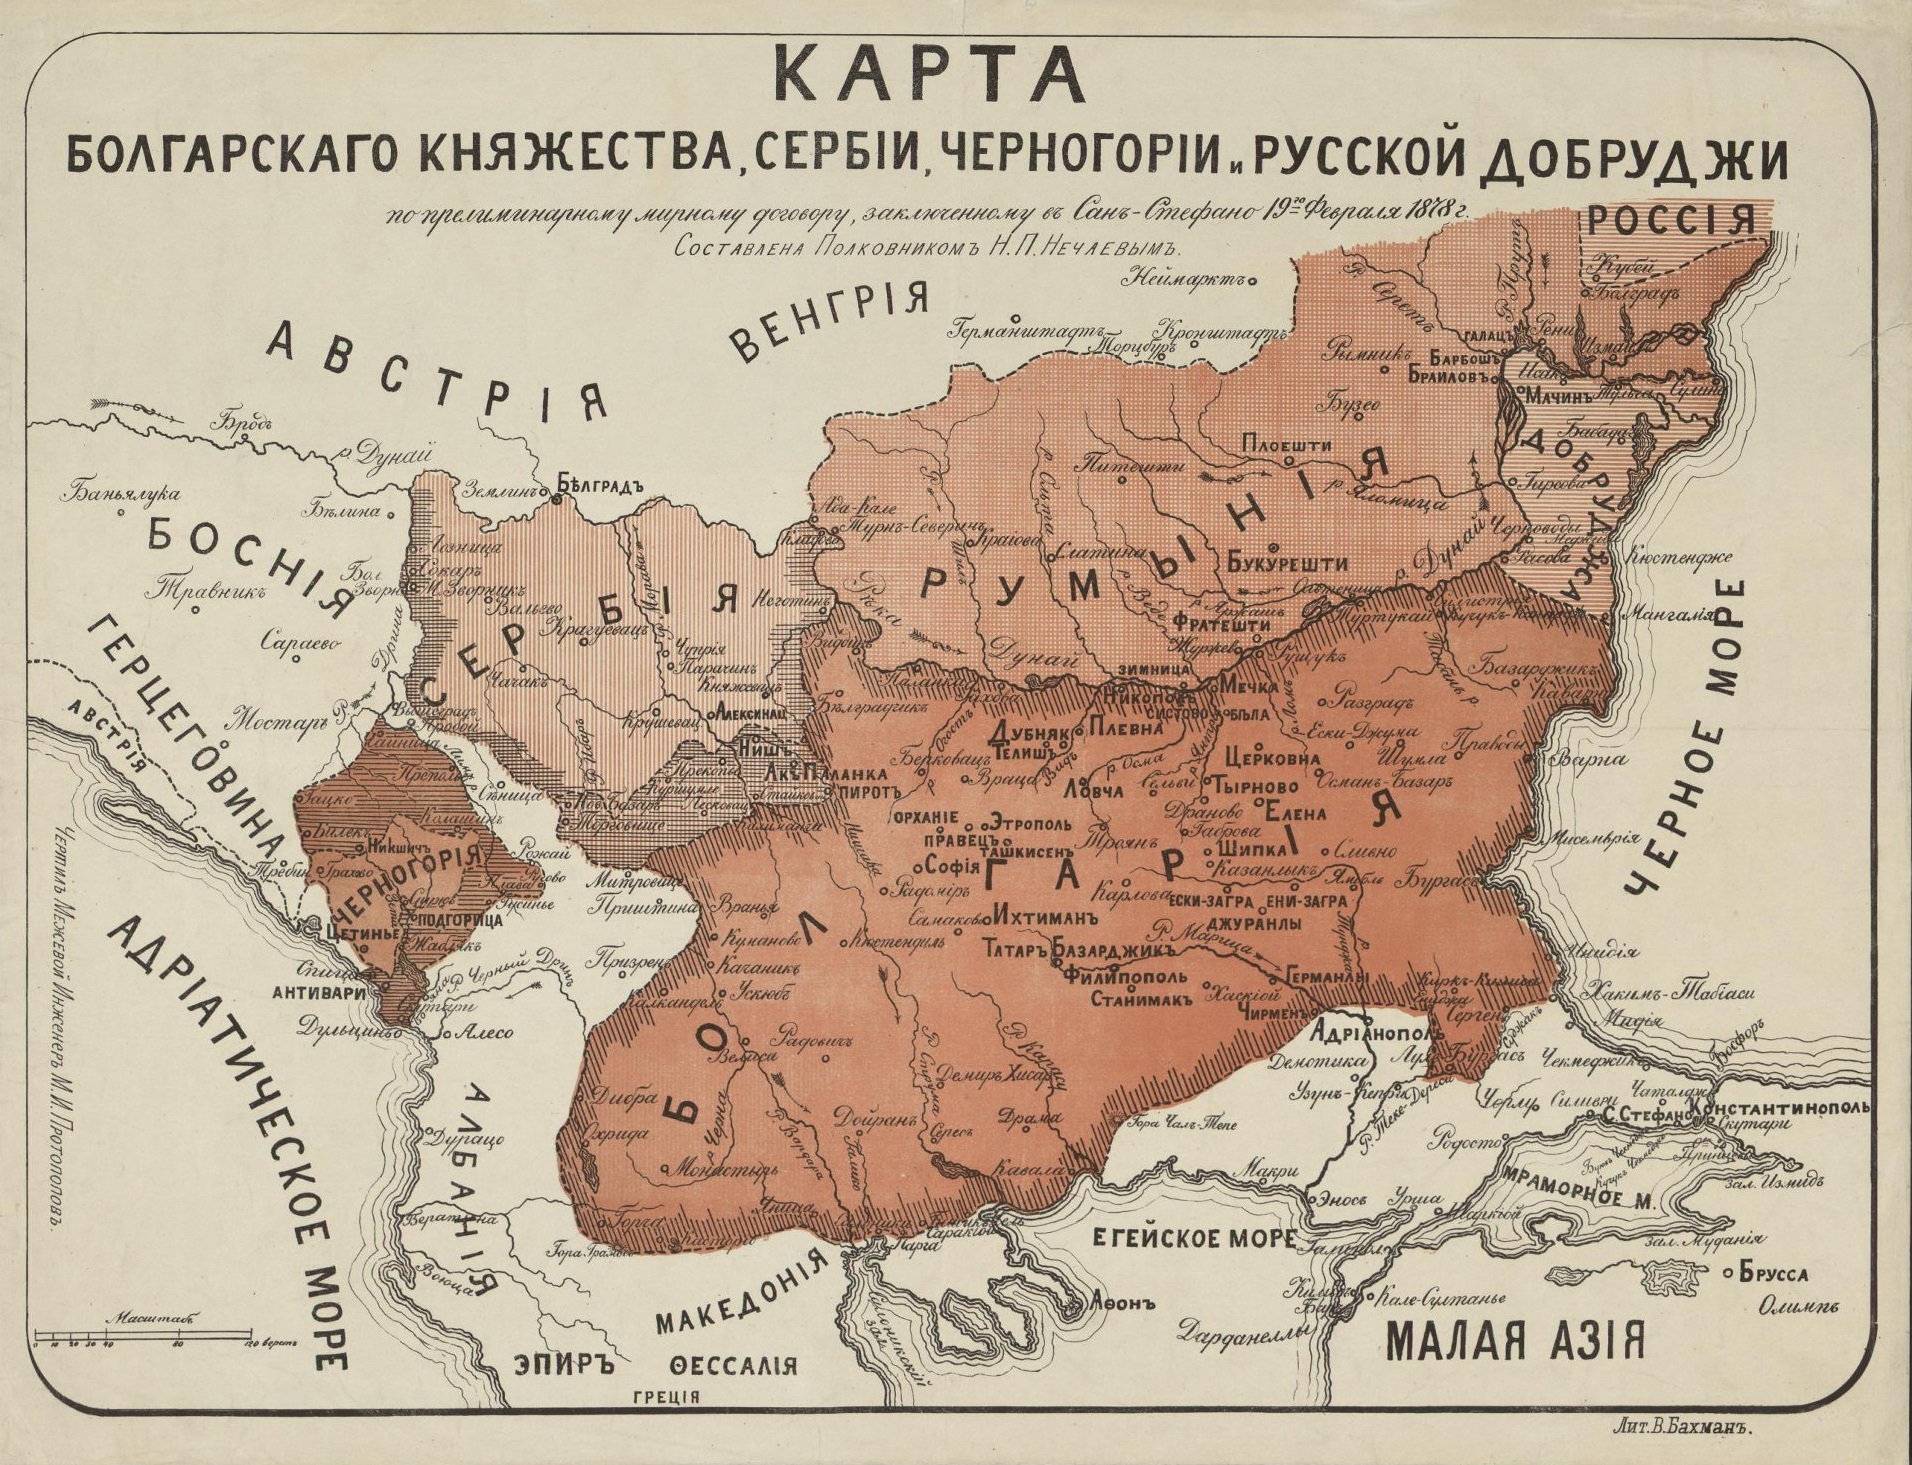
\includegraphics[width=\textwidth]{images/Карта_Балкан_по_Сан-Стефанскому_миру.jpg}}

Что крайне не понравилось империям Европы, а именно Франции, Великобритании и Германии, ведь Сан-Стефанский мир закреплял сильные позиции России в регионе, и большое увеличение влияние в Европе, из-за чего был собран Берлинский конгресс, где остальные Империи пересмотрели итоги договора.

{\centering 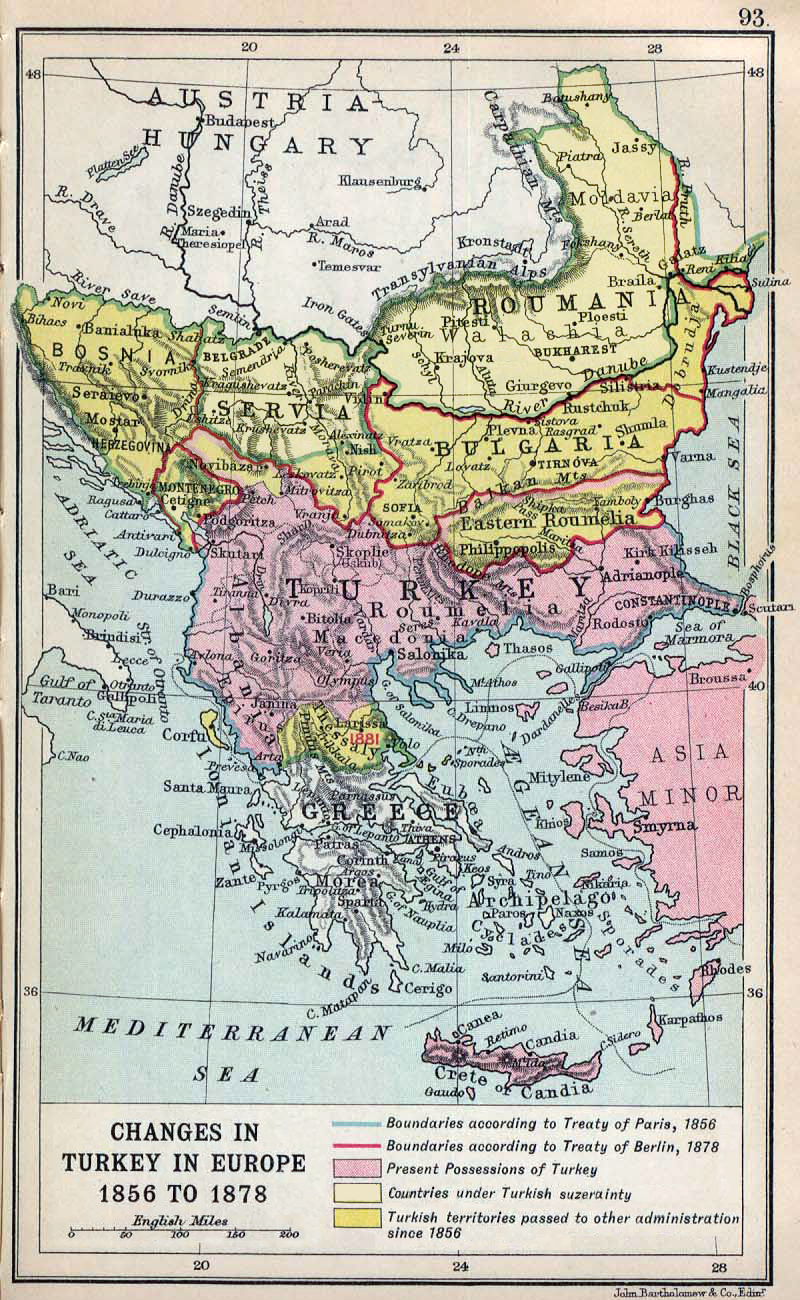
\includegraphics[width=0.5\textwidth]{images/Balkans_1878.png}}

Учитывая выше сказанное Россия на начало XX века несколько потеряло политическое влияние в регионе. Она активно сотрудничала с Сербией и Болгарией, помогая в обучении войск, образуя политические связи, продвигая идеи панславизма, в том числе через позиционирования себя как защитника славян и крестьян в регионе. К концу XIX века влияние над Болгарией было несколько утеряно, и основным мостом в регион оставалась Сербия. Великобритания же следила за тем, чтобы влияние России на Балканах не усиливалось, поддерживая Австро-Венгрию и Османскую империю.